This 3rd Edition of the \emph{Peeragogy Handbook} is dedicated to one of
our most convivial -- indeed, lovable -- volunteers. George Brett was a
quiet and learned man with a sense of fun. His mail art name was geORge
and for a while he was known by many online for the selfies he took with
his yellow rubber duckie. Far from being a full-time funster, George has
been involved in expanding the educational uses of the Internet since
before it was the Internet, both in his work with government
institutions and his many online volunteer activities. He gifted the
Peeragogy project not only with his knowledge and labor, but with his
warmth and fun. We miss him.

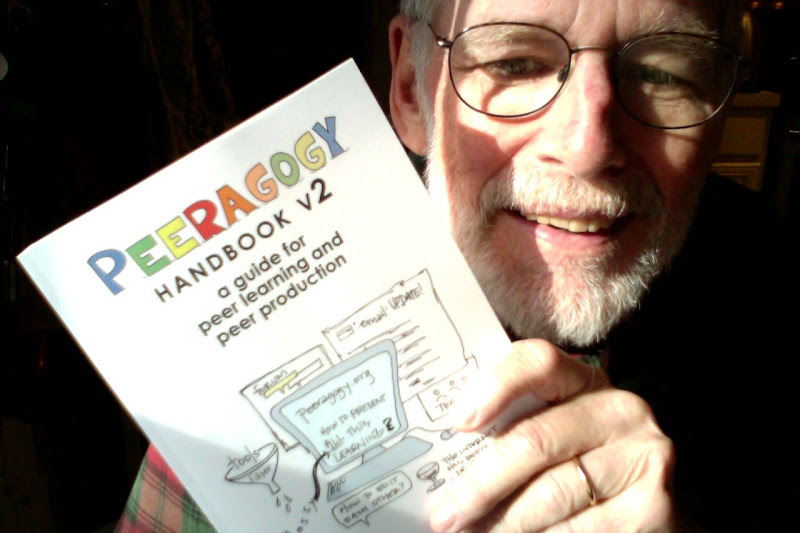
\includegraphics{../pictures/george.jpg}

The Second Edition of the \emph{Handbook} came out two years ago. We've
kept at it since then. This time around, we're kicking things off with a
short workbook that contains a concise guide to the who, what, when,
where, how and why of peeragogy. We've thoroughly revised the pattern
catalog at the heart of the book, added more case studies, and made
numerous small improvements to the text (and the typesetting!)
throughout.
